\section{Implementation}

\begin{figure}[ht]
  \centering
  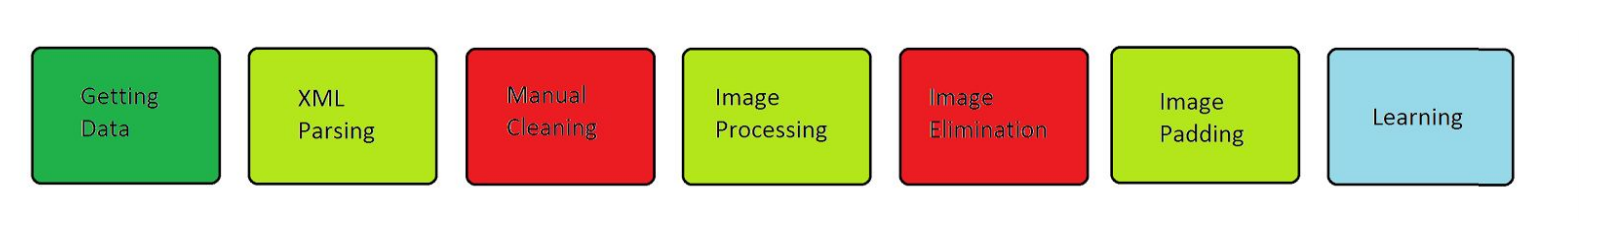
\includegraphics[width=\textwidth]{images/Timeline.png}
  \caption{
    Timeline of activities of this project, flowing from left to right.  The
    yellow-green boxes represent places where we processed our data to be in a
    different format.  The red boxes signify removing unclean data from the
    dataset.
    }
  \label{fig:timeline}
\end{figure}

\subsection{Preprocessing}
After contacting the LDS Church, and signing a non-disclosure agreement we recieved the indexing data from the church. The data that was provided by the church was in a series of xml files that contained the data per each record on a census page and a series of images of each census record.  We learned and designed a xml parser that extracted values from nodes, checked headers, and  accessed attributes.  Learning how to parse xml was necessary, the xml files contained the labels and bounding box information for an image that pertains to the label.  Three xml files were parsed with different parsing routines.  After parsing the files, statistical analysis was ran on the data that was collected.  Several trends were observed, an important one is that the xml file labeled ''truth'' had the highest percentage of correct answers whenever there was a conflict with another xml file results. It was concluded that instead of running a majority vote to determine the true label we would use the labels from truth.xml as the labels. 

Image processing was done to extract the letter according to the bounding box's specifications.  Padding was then implemented on the images to get all the images to a uniform size.  The perspective labels were then placed with the newly created subimages.  Please see Figure~\ref{fig:goodAndBad}. It’s important to note that we have images in our database that may skew the classifier.

For classifiers such as SVM or Averaged Perceptron these erroneous images would be seen as noise and would affect the overall classifier's final results.  We are unsure on how badly these erroneous images would affect deep learning algorithms such as MLP or CNN.   Perhaps these real world errors will have a more negative effect of overall classifier or maybe we will have a better result than the traditional linear classifiers.

\subsection{Data Cleaning}
During the xml parsing and image processing we eliminated/cleaned our data to remove any data that wasn’t complete i.e. we had the labels but not the bounding box where we could extract the subimages. Analysis was performed on the parsed bounding box data.  It was determined that some of the subimages that would be created from the bounding box would be too small or too big to use.  These records and labels were eliminated, leaving around 70,000 subimages that would form our  test, validation, and training sets.  

\subsection{Learning}
We implemented Perceptron, Averaged Perceptron, SVM, and Logistic Regression from scratch, using the Theano Library.  This was done by implement the individual loss functions and then run minibatch stocastic sub-gradient decent to find the weight vector that best classfied the data.  For the implementation of CNN we began with the CNN code to classify the MNIST data on deeplearning.net.  From this example we modified the code to work with our dataset and implemented cross validation to selected the best number of kernels for our CNN to use.


